\documentclass{article}
\title{Sprawozdanie 2 \\ Testowanie opracowanej metody heurystycznej}
\date{2018-06-01}
\author{Mateusz Babiaczyk, Bartosz Nawrotek}
\usepackage[utf8]{inputenc}
\usepackage[T1]{fontenc}
\usepackage{graphicx}
\usepackage{float}
\graphicspath{ {Wykresy/} }
\usepackage{geometry}
 \geometry{
 a4paper,
 total={170mm,257mm},
 left=20mm,
 top=20mm,
 }

\begin{document}
\maketitle
\section{Zmiany w algorytmie}  
Po zaimplementowaniu algorytmu i zauważeniu jego słabych osiągnięć, doszliśmy do wniosku by wprowadzić zmiany w naszym algorytmie. 
\subsection{Mutacje}
\subsection{Krzyżowanie}
Krzyżowanie zaczyna się w dokładnie taki sam sposób jak było w naszym pierwotnym algorytmie, a mianowicie od pewnego wylosowanego przedziału przepisuje oligonukleotydy do nowo tworzonego osobnika (kopiuje wycinek i wkleja go do nowego osobnika) z wybranego osobnika z populacji rodzicielskiej. Następnie uzupełniany jest koniec osobnika wartościami z innego osobnika z populacji rodzicielskiej, uważając oczywiście by dany oligonukleotyd nie został powtórzony. W ten sam sposób zostaje uzupełniony początek osobnika z nowej populacji. \\ Wszystkie oligonukleotydy które nie zostały dodane (na wskutek dodawania ich z innego osobnika który za punktem cięcia mógł mieć oligounkloeotyd taki sam jak drugi osobnik użyty do krzyżowania pomiędzy punktami cięcia) zostają dodane, każdy osobno, w miejsce w którym funkcja celu będzie najniższa. Dzięki takiemu nakierowaniu, nadal mieliśmy pewną dużą losowość przez krzyżowanie między losowymi punktami cięcia (która jest ważna w algorytmie genetycznym), a jednocześnie algorytm szybciej zbiegał do wartości optymalnych, tym samy dając lepsze rezultaty w krótszym czasie.
\subsection{Kodowanie}
\section{Testy}
\subsection{Wyniki algorytmu dla błędów negatywnych, losowych}
\begin{figure}[H]
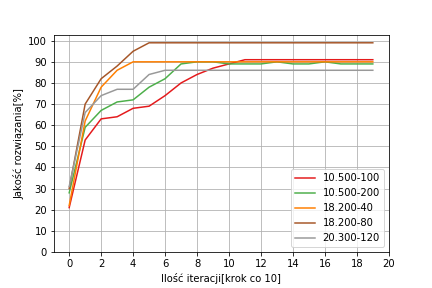
\includegraphics[width=0.5\textwidth]{neg-los1.png}
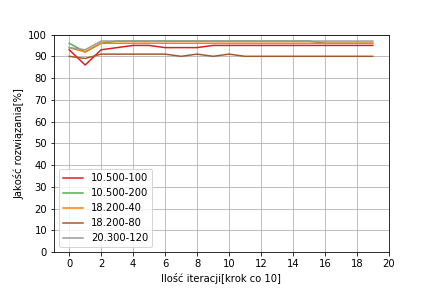
\includegraphics[width=0.5\textwidth]{neg-los-greedy1.png}
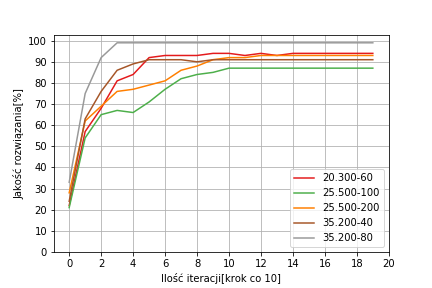
\includegraphics[width=0.5\textwidth]{neg-los2.png}
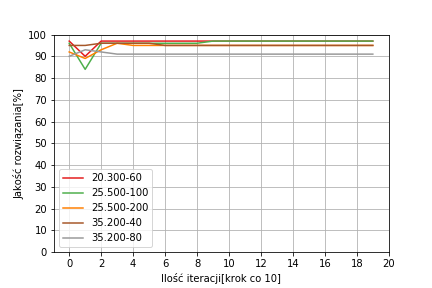
\includegraphics[width=0.5\textwidth]{neg-los-greedy2.png}
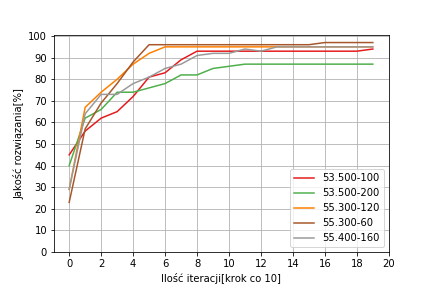
\includegraphics[width=0.5\textwidth]{neg-los3.png}
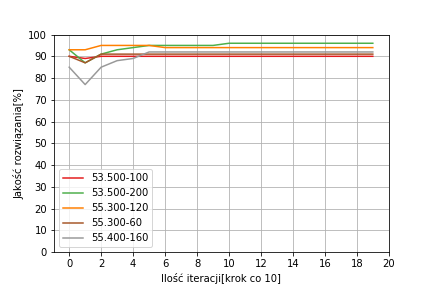
\includegraphics[width=0.5\textwidth]{neg-los-greedy3.png}
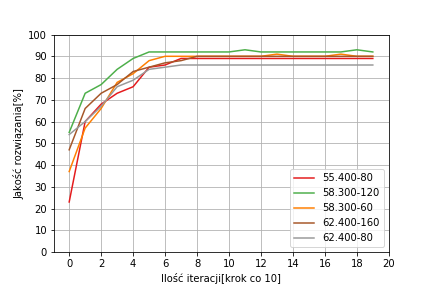
\includegraphics[width=0.5\textwidth]{neg-los4.png}
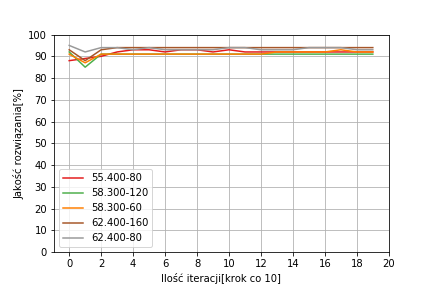
\includegraphics[width=0.5\textwidth]{neg-los-greedy4.png}
\caption{Porównanie algorytmu dla błędów negatywnych, losowych bez oraz z wykorzystanym osobnikiem wygenerownym przez algorytm zachłanny w zależności od ilości iteracji}
\end{figure}
\begin{figure}[H]
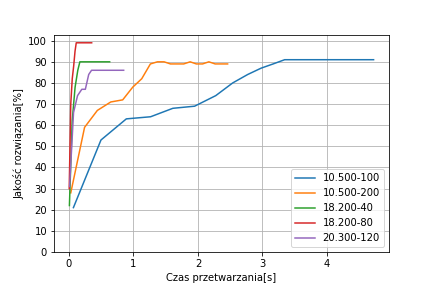
\includegraphics[width=0.5\textwidth]{Czasneg-los1.png}
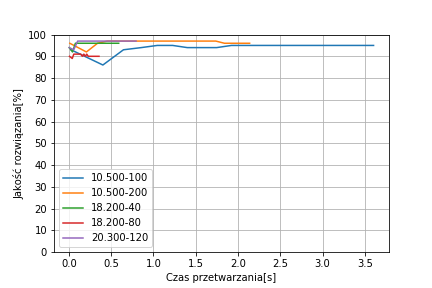
\includegraphics[width=0.5\textwidth]{Czasneg-los-greedy1.png}
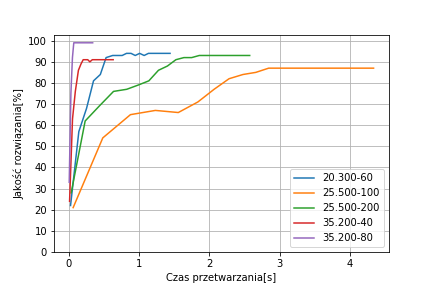
\includegraphics[width=0.5\textwidth]{Czasneg-los2.png}
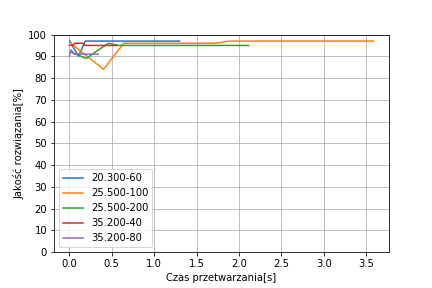
\includegraphics[width=0.5\textwidth]{Czasneg-los-greedy2.png}
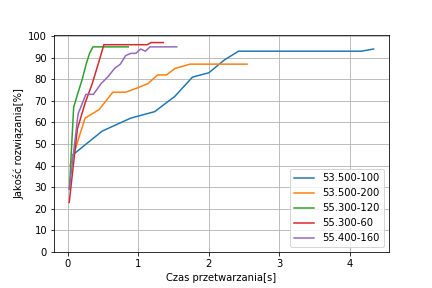
\includegraphics[width=0.5\textwidth]{Czasneg-los3.png}
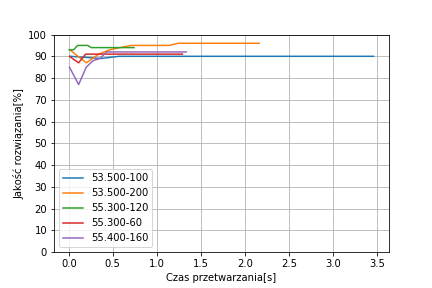
\includegraphics[width=0.5\textwidth]{Czasneg-los-greedy3.png}
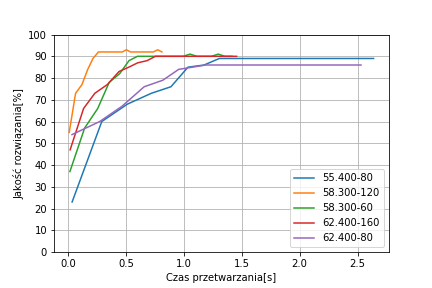
\includegraphics[width=0.5\textwidth]{Czasneg-los4.png}
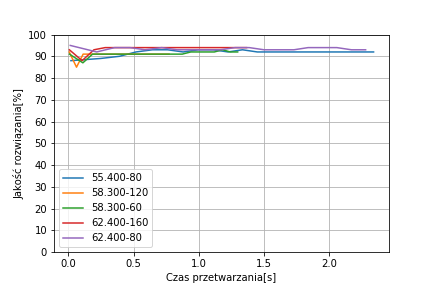
\includegraphics[width=0.5\textwidth]{Czasneg-los-greedy4.png}
\caption{Porównanie algorytmu dla błędów negatywnych, losowych bez oraz z wykorzystanym osobnikiem wygenerownym przez algorytm zachłanny w zależności od czasu przetwarzania}
\end{figure}
Jak widać, dla błędów negatywnych losowych algorytm otrzymuje rozwiązanie o średniej dokładności 90%. W algorytmie z początkowym algorytmem zachłannym (wykresy po prawej) widać że otrzymuje on średnio lepsze wyniki z prostej przyczyny początkowego uszeregowania które ma bardzo dobrą jakość rozwiązania. Powodem tego są rodzaje testów, które bardzo dobrze są rozwiązywane przez algorytm zachłanny. Nie zmienia to jednak faktu, że algorytm bez początkowego rozpoczęcia zachłannego uzyskuje podobne wyniki, a funkcja poprawnie zbiega do celu.
\subsection{Wyniki algorytmu dla błędów negatywnych na końcach sekwencji}
\begin{figure}[H]
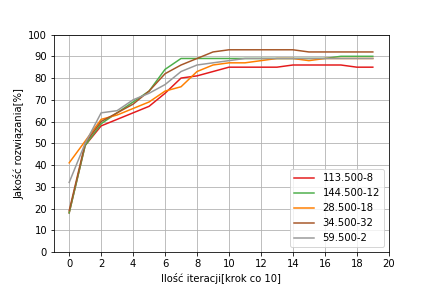
\includegraphics[width=0.5\textwidth]{neg-pow1.png}
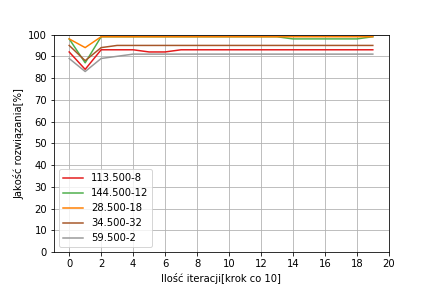
\includegraphics[width=0.5\textwidth]{neg-pow-greedy1.png}
\caption{Porównanie algorytmu dla błędów negatywnych na końcach sekwencji bez oraz z wykorzystanym osobnikiem wygenerownym przez algorytm zachłanny w zależności od ilości iteracji}
\end{figure}
\begin{figure}[H]
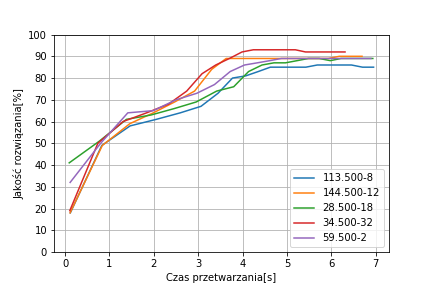
\includegraphics[width=0.5\textwidth]{Czasneg-pow1.png}
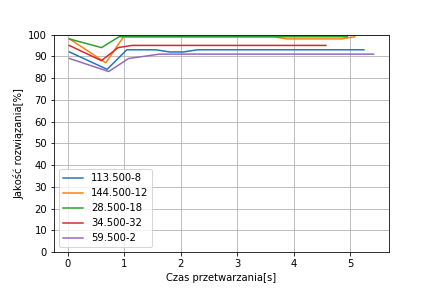
\includegraphics[width=0.5\textwidth]{Czasneg-pow-greedy1.png}
\caption{Porównanie algorytmu dla błędów negatywnych na końcach sekwencji bez oraz z wykorzystanym osobnikiem wygenerownym przez algorytm zachłanny w zależności od czasu przetwarzania}
\end{figure}
W przypadku  błędów negatywnych na końcach sekwencji wyniki są zbliżone do błędów negatywnych losowych i zachowują taką samą własność.
\subsection{Wyniki algorytmu dla błędów pozytywnych, losowych}
\begin{figure}[H]
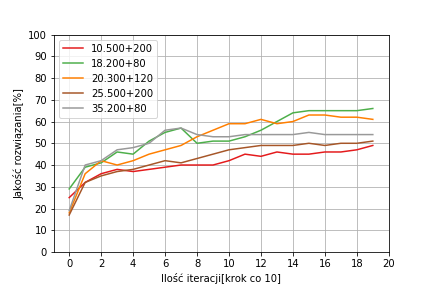
\includegraphics[width=0.5\textwidth]{poz-los1.png}
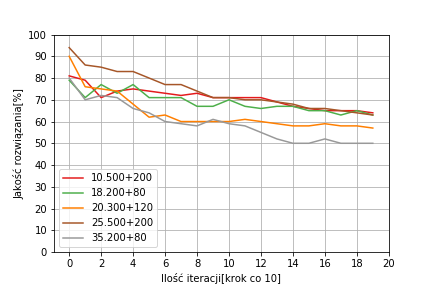
\includegraphics[width=0.5\textwidth]{poz-los-greedy1.png}
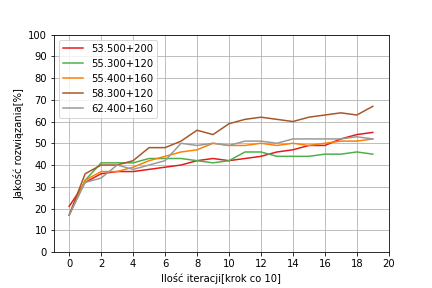
\includegraphics[width=0.5\textwidth]{poz-los2.png}
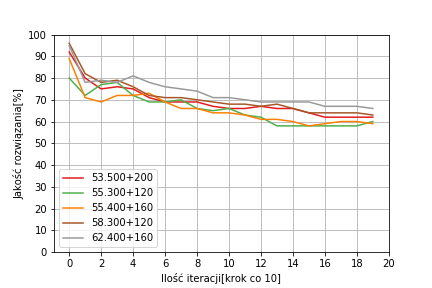
\includegraphics[width=0.5\textwidth]{poz-los-greedy2.png}
\caption{Porównanie algorytmu dla błędów pozytywnych, losowych bez oraz z wykorzystanym osobnikiem wygenerownym przez algorytm zachłanny w zależności od ilości iteracji}
\end{figure}
\begin{figure}[H]
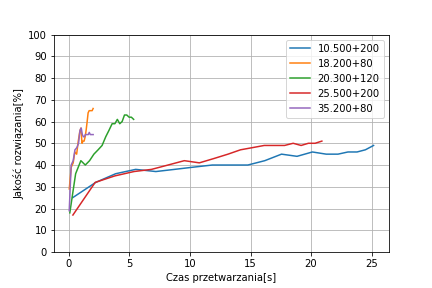
\includegraphics[width=0.5\textwidth]{Czaspoz-los1.png}
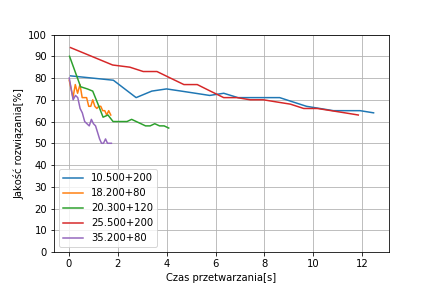
\includegraphics[width=0.5\textwidth]{Czaspoz-los-greedy1.png}
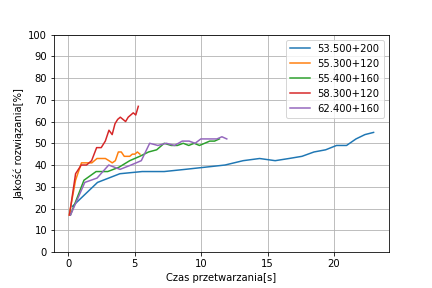
\includegraphics[width=0.5\textwidth]{Czaspoz-los2.png}
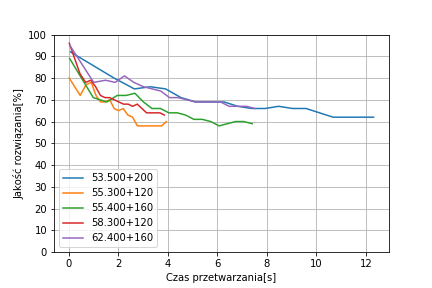
\includegraphics[width=0.5\textwidth]{Czaspoz-los-greedy2.png}
\caption{Porównanie algorytmu dla błędów pozytywnych, losowych bez oraz z wykorzystanym osobnikiem wygenerownym przez algorytm zachłanny w zależności od czasu przetwarzania}
\end{figure}
Dla błędów pozytywnych losowych nasz algorytm nie działa już tak dobrze. Jak widać algorytm bez początku zachłannego uzyskuje średnie wyniki w okolicach 60%. Jest do dość słaby wynik. Dodatkowo algorytm z początkiem zachłannym tylko pogarsza swoje wyniki po lepszym wyniku zachłannym, żeby ostatecznie dojść do prawie takiego samego wyniku jak algorytm bez początku zachłannego.  
\subsection{Wyniki algorytmu dla błędów pozytywnych, na końcach sekwencji}
\begin{figure}[H]
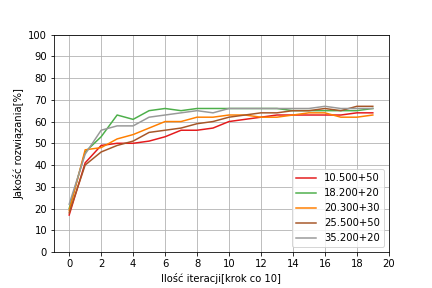
\includegraphics[width=0.5\textwidth]{poz-oli1.png}
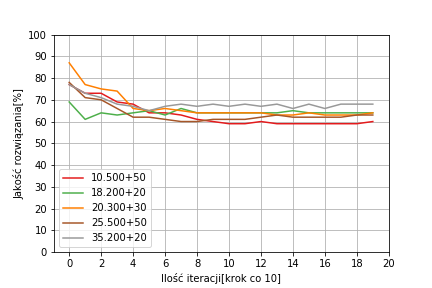
\includegraphics[width=0.5\textwidth]{poz-oli-greedy1.png}
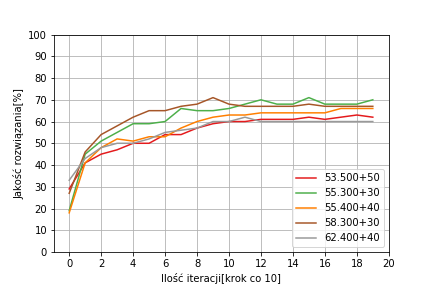
\includegraphics[width=0.5\textwidth]{poz-oli2.png}
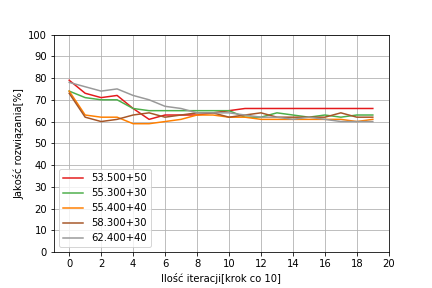
\includegraphics[width=0.5\textwidth]{poz-oli-greedy2.png}
\caption{Porównanie algorytmu dla błędów pozytywnych na końcach sekwencji bez oraz z wykorzystanym osobnikiem wygenerownym przez algorytm zachłanny w zależności od ilości iteracji}
\end{figure}
\begin{figure}[H]
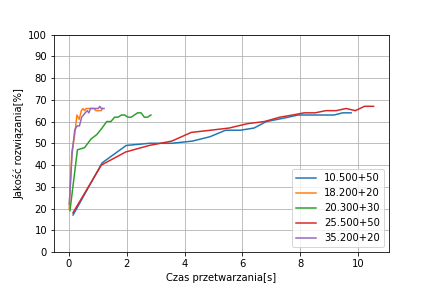
\includegraphics[width=0.5\textwidth]{Czaspoz-oli1.png}
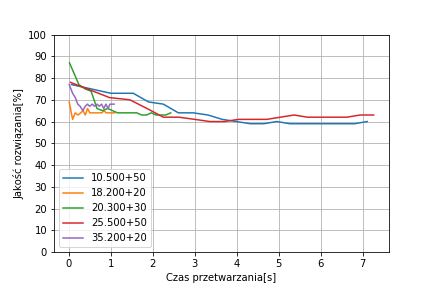
\includegraphics[width=0.5\textwidth]{Czaspoz-oli-greedy1.png}
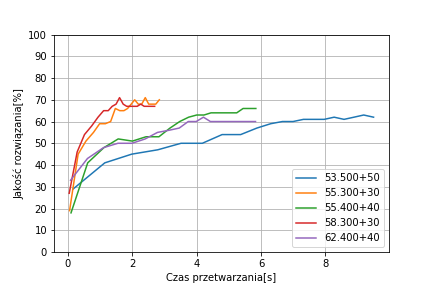
\includegraphics[width=0.5\textwidth]{Czaspoz-oli2.png}
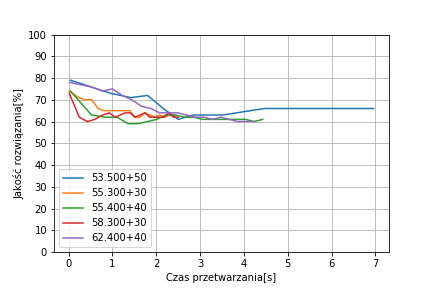
\includegraphics[width=0.5\textwidth]{Czaspoz-oli-greedy2.png}
\caption{Porównanie algorytmu dla błędów pozytywnych na końcach sekwencji bez oraz z wykorzystanym osobnikiem wygenerownym przez algorytm zachłanny w zależności od czasu przetwarzania}
\end{figure}
Ostatnią kategorią są błędy pozytywne z przekłamaniami na końcach oligonukleotydów. Jak widać radzi on sobie odrobinę lepiej niż dla błędów pozutywnych losowych, dodatkowo algorytm z rozpoczęciem zachłannym nie maleje aż tak bardzo (algorytm zachłanny ma większe problemy z optymalnym ustawieniem i jego wykonanie nie powoduje od razu ustawienia pierwszej iteracji na wysokości 90-95%, a nieco niżej na 70-80%).
\section{Wnioski}
\end{document}


